\section{Complexity Estimation} \label{sec:complexity_estimation}

A region is said to be complex, if it contains more than one unique label. Otherwise, a region is simple. Since the data within a region already represents a cluster, the existence of multiple classes indicates a more complex decision boundary. On that basis we differentiate how a region is processed in the subsequent services of the pipeline. Furthermore, the complexity state of a region may vary, depending on the scope it is observed. Note that since the projection matrix $\bm{M}$ is initialized with the same values in every $L_m$, all hashes that were computed by $h$ are globally comparable. This means that similar data points from different datasets, e.g. $\bm{x}_i \in D_1$ and $\bm{x}_j^* \in D_2$ may be hashed to the same region $h(\bm{x}_i) = h(\bm{x}^*_j)$. However, it is also possible that that the corresponding labels $y_i \in D_1$ and $y^*_j \in D_2$ are not equal and therefore lead to a different global view on that region's complexity state. Given that, the complexity estimation module acts as a bridge between the local and global components and answers the question, which regions are considered to be complex in a global context. 

\begin{algorithm}
   \caption{Creating a global complexity state by combining local complexity states}
   \label{alg:complexity_estimation}
   \algsetup{indent=2em}

   \begin{algorithmic}[1]
         \REQUIRE Regions $R_{\text{in}}$
         \ENSURE Regions $R_{\text{out}}$
         \STATE $R_{\text{out}} \leftarrow $ new Set
         \STATE $m \leftarrow$ getID() \COMMENT{current local infrastructure identifier}
         \FORALL{$r$ in $R$}
            \STATE $k_\gamma \leftarrow \text{concatenate}(p_y, r)$
            \STATE $Y_r \leftarrow PDB_{L_m}[k_\gamma]$
            \STATE $k_\delta \leftarrow \text{concatenate}(p_y, r, m)$
            \STATE $PDB_G[k_\delta] \leftarrow Y_r$
            \STATE $S \leftarrow$ new Set
            \FORALL{$m$ in $\{1, \dots, M\}$}
               \STATE $k_\delta \leftarrow \text{concatenate}(p_y, r, m)$
               \STATE $Y_r \leftarrow PDB_G[k_\delta]$
               \STATE insert $Y_r$ into $S$
            \ENDFOR
            \IF{$|S| > 1$} 
               \STATE $c_r \leftarrow 1$ 
            \ELSE 
               \STATE $c_r \leftarrow 0$ 
            \ENDIF
            \STATE $k_\kappa \leftarrow \text{concatenate}(p_c, r)$
            \IF{$PDB_G[k_\kappa] \neq c_r$}
               \STATE $PDB_G[k_\kappa] \leftarrow c_r$
               \STATE insert $r$ into $R_{\text{out}}$
            \ENDIF
         \ENDFOR
         \RETURN $R_{\text{out}}$
   \end{algorithmic}
\end{algorithm}

First, a set of regions $R$ is received. Then, for each region $r \in R$ the following operations are defined. The set of unique labels $Y_r$ for a particular region has been stored in Algorithm~\ref{alg:indexing} as auxiliary metadata, which is now retrieved by constructing the correspoding key $k_\gamma$. Subsequently, the slot $PDB_{L_m}[k_\gamma]$ is accessed and $Y_r$ is retrieved. In the next step, $Y_r$ has to be stored in the $PDB_G$. Therefore, another key $k_\delta$ is constructed by concatenating the prefix constant $p_y$, the region $r$ and the current local infrastructure identifier $m$, which prevents the collision of information from different infrastructures.

After $Y_r$ is stored on a global level at $PDB_G[k_\delta]$, the label set information for that region from all members in the CIDS is aggregated. That aggregated view is essentially the global complexity state for that region. By iterating over all member identifiers in the CIDS, multiple keys $k_\delta$ are constructed. Each key retrieves the specific label set $Y_r$ of a member and inserts its content into the set $S$. 

After collecting all label sets in $S$, the complexity state is obtained by simply evaluating the cardinality $|S|$. If there is more than one class in a region on a global scope, that is $|S| > 1$, then assign a true value to the global complexity variable $c_r$. Otherwise, assign a false value. In order to store $c_r$, the key $k_\kappa$ is created by concatenating the prefix constant $p_c$ and the region $r$. Note, that $PDB_G[k_\kappa]$ is only updated, if storing $c_r$ changes the state that is already persisted. This is because, if an update is executed, this information has to be propagated to the next service. Thus, in that case, the region $r$ is inserted into $R_{\text{out}}$, which is subsequently sent into the global event channel $C_G$ in order to inform services in all local infrastructures about the update.

\begin{figure}[t]
   \centering
   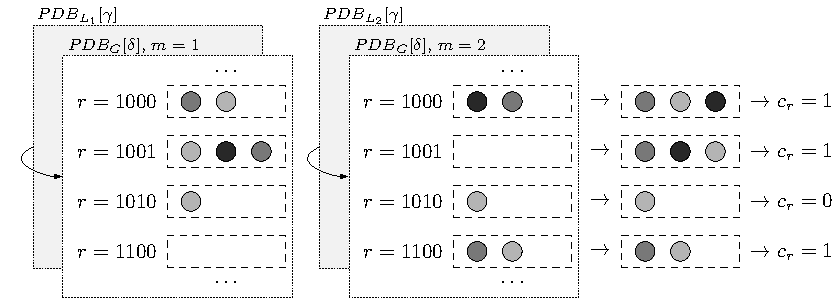
\includegraphics[width=1\linewidth]{tikz/complexity_estimation.pdf}
   \caption{Illustration of the complexity estimation algorithm with two local infrastructures. Each local label set at $PDB_{L_m}[k_\kappa]$ is synchronized into the global pattern database at $PDB_G[k\delta]$, where $k_\delta$ is constructed with $m$. Per region, the union operation is applied on the global label sets, whereupon the complexity is derived from.}  \label{fig:complexity_estimation}
\end{figure}